% Moran process: Hawk-Dove with three individuals, run on dice.
% Shared preamble for the write-on class slides.
%
% Every deck is designed to be projected and annotated live on a tablet:
% whatever takes time to draw is pre-drawn, and whatever the class produces is
% left blank. Compile a deck with `pdflatex main.tex` from its own directory,
% or run `make` in decks/ to build them all.
\documentclass[10pt]{article}

\usepackage[papersize={25.6cm,14.4cm}, margin=1.1cm, bottom=1.5cm,
            footskip=0.75cm]{geometry}
\usepackage[T1]{fontenc}
\usepackage[default]{sourcesanspro}
\usepackage{newtxsf}
\usepackage{tikz}
\usepackage{amsmath}
\usepackage{parskip}
\usepackage{fancyhdr}
\usetikzlibrary{arrows.meta, positioning, calc}

\setlength{\parindent}{0pt}

% Catppuccin Latte, the palette the course site uses in its light theme, so a
% deck on the projector looks like the pages the students read.
\definecolor{inkbg}{HTML}{EFF1F5}      % base
\definecolor{inksurface}{HTML}{E6E9EF} % mantle
\definecolor{inkfaint}{HTML}{CCD0DA}   % surface2, for rules and empty boxes
\definecolor{inktext}{HTML}{4C4F69}    % text
\definecolor{inkgrey}{HTML}{8C8FA1}    % overlay1, for anything secondary
\definecolor{inkblue}{HTML}{7287FD}    % lavender, the primary accent
\definecolor{inkteal}{HTML}{179299}    % teal
\definecolor{inkred}{HTML}{FE640B}     % peach, for whatever wants attention
\definecolor{inkmauve}{HTML}{8839EF}   % mauve

\pagecolor{inkbg}
\color{inktext}

% A box to write a number into. White against the tinted page, so it reads as
% somewhere to write rather than as part of the printed material.
\newcommand{\blank}[1][1.6]{%
  \tikz[baseline=(current bounding box.base)]{%
    \draw[inkfaint, line width=0.7pt, rounded corners=2pt, fill=white]
      (0,-0.18) rectangle (#1,0.62);}}

% A ruled area to work in. Faint dots keep handwriting level on a tablet.
\newcommand{\workspace}[2]{%
  \begin{tikzpicture}
    \draw[inkfaint, line width=0.7pt, rounded corners=3pt, fill=white]
      (0,0) rectangle (#1,#2);
    \foreach \gx in {0.5,1.0,...,#1}{%
      \foreach \gy in {0.5,1.0,...,#2}{%
        \fill[inkfaint] (\gx,\gy) circle (0.5pt);}}
  \end{tikzpicture}}

% A panel for material that is printed rather than written on.
\newcommand{\panel}[2]{%
  \begin{tikzpicture}
    \draw[inkfaint, line width=0.7pt, rounded corners=3pt, fill=inksurface]
      (0,0) rectangle (#1,#2);
  \end{tikzpicture}}

% An empty payoff grid. #1 is the list of action names, #2 is drawn afterwards
% so a page can add its own marks.
\newcommand{\payoffgrid}[2]{%
  \begin{tikzpicture}[scale=1.0, every node/.style={transform shape}]
    \foreach \name [count=\j from 0] in {#1}{%
      \node[font=\bfseries, text=inkblue] at (\j*2.7+1.35,0.55) {\name};
      \node[font=\bfseries, text=inkblue] at (-1.15,-\j*2-1) {\name};
      \foreach \k [count=\i from 0] in {#1}{%
        \draw[inkfaint, line width=0.7pt, fill=white]
          (\j*2.7,-\i*2) rectangle (\j*2.7+2.7,-\i*2-2);}}
    #2
  \end{tikzpicture}}

% The five actions on a pentagon. Each action beats the one next to it and the
% one across from it, so the two winning cycles are drawn as separate panels:
% ten labelled arrows on one diagram is a tangle nobody can read from the back
% of the room.
\newcommand{\rpslscycle}[3]{%
  \begin{tikzpicture}[scale=1.0, every node/.style={transform shape},
      >={Stealth[length=2.6mm]},
      action/.style={circle, draw=inkfaint, line width=1pt, fill=white,
                     text=inktext, minimum size=1.7cm, inner sep=1pt,
                     font=\small\bfseries},
      beats/.style={->, line width=1.2pt, shorten >=3pt, shorten <=3pt,
                    draw=#1},
      word/.style={font=\scriptsize, fill=inkbg, inner sep=1.6pt, text=#1,
                   sloped, pos=#2}]
    \foreach \name/\angle in {Rock/90, Lizard/18, Spock/-54,
                              Scissors/-126, Paper/162}{%
      \node[action] (\name) at (\angle:3.1) {\name};}
    \foreach \winner/\loser/\said in {#3}{%
      \draw[beats] (\winner) -- node[word] {\said} (\loser);}
  \end{tikzpicture}}

% Running header: the deck name on the left, the page's own step on the right.
% Each deck sets its name once with \deckname.
\newcommand{\deck}{}
\newcommand{\deckname}[1]{\renewcommand{\deck}{#1}}
\newcommand{\slidehead}[1]{%
  {\small\color{inkgrey}%
   \tikz[baseline=-0.5ex]{\fill[inkblue, rounded corners=1pt]
     (0,0) rectangle (0.22,0.22);}\;\deck
   \hfill \color{inkblue}\bfseries #1}\par
  {\color{inkblue}\rule{\linewidth}{1pt}}\par\vspace{0.35em}}

\pagestyle{fancy}
\fancyhf{}
\renewcommand{\headrulewidth}{0pt}
\fancyfoot[R]{\small\color{inkgrey}\thepage}

% Deck title pages, which carry no header and no page number.
\newcommand{\titleslide}[3]{%
  \thispagestyle{empty}%
  \begin{center}
    \vspace*{\fill}
    {\Huge\bfseries\color{inkblue} #1}\\[0.7em]
    {\LARGE\color{inkgrey} #2}\\[2.4em]
    #3
    \vspace*{\fill}
  \end{center}}

% One step of the plan on a title page.
\newcommand{\stepbox}[3]{%
  \node[draw=inkblue, line width=0.9pt, rounded corners=4pt, fill=white,
        minimum width=6cm, minimum height=1.7cm, align=center,
        text=inktext] (#1) at (#2,0) {#3};}


% The birth-death chain on the number of hawks, with the transitions left
% blank. Gains run along the top, losses along the bottom.
\newcommand{\birthdeath}{%
  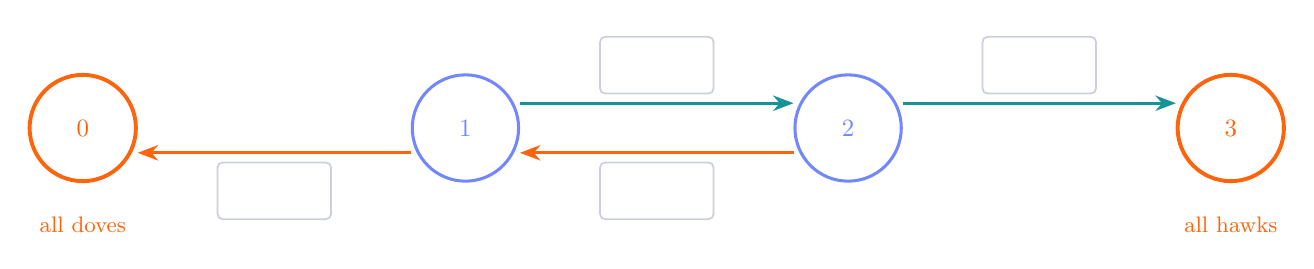
\begin{tikzpicture}[scale=0.9, every node/.style={transform shape},
      >={Stealth[length=2.6mm]},
      state/.style={circle, draw=inkblue, line width=1.1pt, fill=white,
                    text=inkblue, minimum size=1.5cm, font=\bfseries,
                    inner sep=0pt},
      absorb/.style={state, draw=inkred, text=inkred, line width=1.4pt},
      gain/.style={->, line width=1.1pt, draw=inkteal},
      loss/.style={->, line width=1.1pt, draw=inkred}]
    \node[absorb] (s0) at (0,0) {$0$};
    \node[state]  (s1) at (5.4,0) {$1$};
    \node[state]  (s2) at (10.8,0) {$2$};
    \node[absorb] (s3) at (16.2,0) {$3$};
    \draw[gain] ([yshift=3.5mm]s1.east) --
      node[above, font=\small] {\blank[1.6]} ([yshift=3.5mm]s2.west);
    \draw[gain] ([yshift=3.5mm]s2.east) --
      node[above, font=\small] {\blank[1.6]} ([yshift=3.5mm]s3.west);
    \draw[loss] ([yshift=-3.5mm]s1.west) --
      node[below, font=\small] {\blank[1.6]} ([yshift=-3.5mm]s0.east);
    \draw[loss] ([yshift=-3.5mm]s2.west) --
      node[below, font=\small] {\blank[1.6]} ([yshift=-3.5mm]s1.east);
    \node[below=0.35cm of s0, font=\small, text=inkred] {all doves};
    \node[below=0.35cm of s3, font=\small, text=inkred] {all hawks};
  \end{tikzpicture}}

\deckname{Moran process}

\begin{document}

\titleslide{Moran process}{Three individuals, two dice, one survivor}{%
    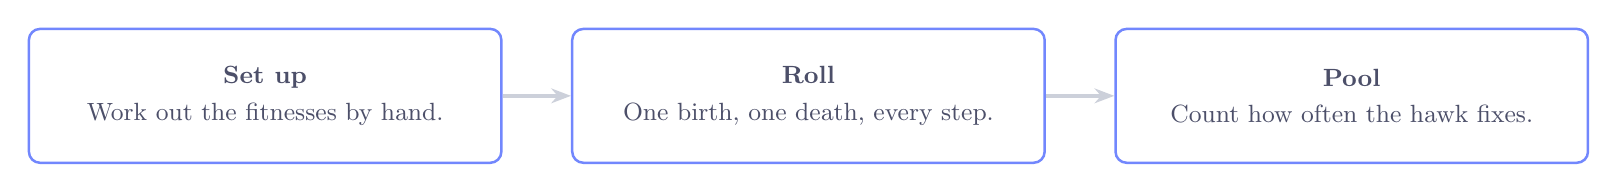
\begin{tikzpicture}[font=\small]
      \stepbox{s0}{0.0}{\textbf{Set up}\\[0.25em]
        Work out the fitnesses by hand.}
      \stepbox{s1}{6.9}{\textbf{Roll}\\[0.25em]
        One birth, one death, every step.}
      \stepbox{s2}{13.8}{\textbf{Pool}\\[0.25em]
        Count how often the hawk fixes.}
      \draw[-{Stealth[length=2.5mm]}, inkfaint, line width=1.2pt] (s0) -- (s1);
      \draw[-{Stealth[length=2.5mm]}, inkfaint, line width=1.2pt] (s1) -- (s2);
    \end{tikzpicture}

    \vspace{2.4em}

    {\large Pairs playing: \blank[2.2] \hspace{2cm}
     Starting state: one hawk, two doves}}

\newpage
\slidehead{Hawk-Dove, and where it can end}


\begin{minipage}[c]{0.34\linewidth}
\begin{center}
\payoffgrid{Hawk, Dove}{%
  \node at (1.35,-1) {\Large $0$};
  \node at (4.05,-1) {\Large $3$};
  \node at (1.35,-3) {\Large $1$};
  \node at (4.05,-3) {\Large $2$};}
\end{center}
\end{minipage}
\hfill
\begin{minipage}[c]{0.62\linewidth}
\raggedright
{\large Four resources to share. Two hawks get \blank[1.2] each; a hawk meeting
a dove takes \blank[1.2] to the dove's \blank[1.2]; two doves split them
\blank[1.2] each.}
\end{minipage}

\vspace{0.35cm}

\begin{center}
\birthdeath
\end{center}

\vspace{0.1cm}

{\small\color{inkgrey} The number of hawks. Along the top a hawk is born; along
the bottom one dies. The two ends are absorbing, so the process stops only once
one type is gone.}

\newpage
\slidehead{How fit is each type?}

\vspace{0.5cm}

{\large A type's fitness counts what it scores against everyone \emph{else} in
the population, so it never plays itself.}

\vspace{0.7cm}

\hspace{0.3cm}
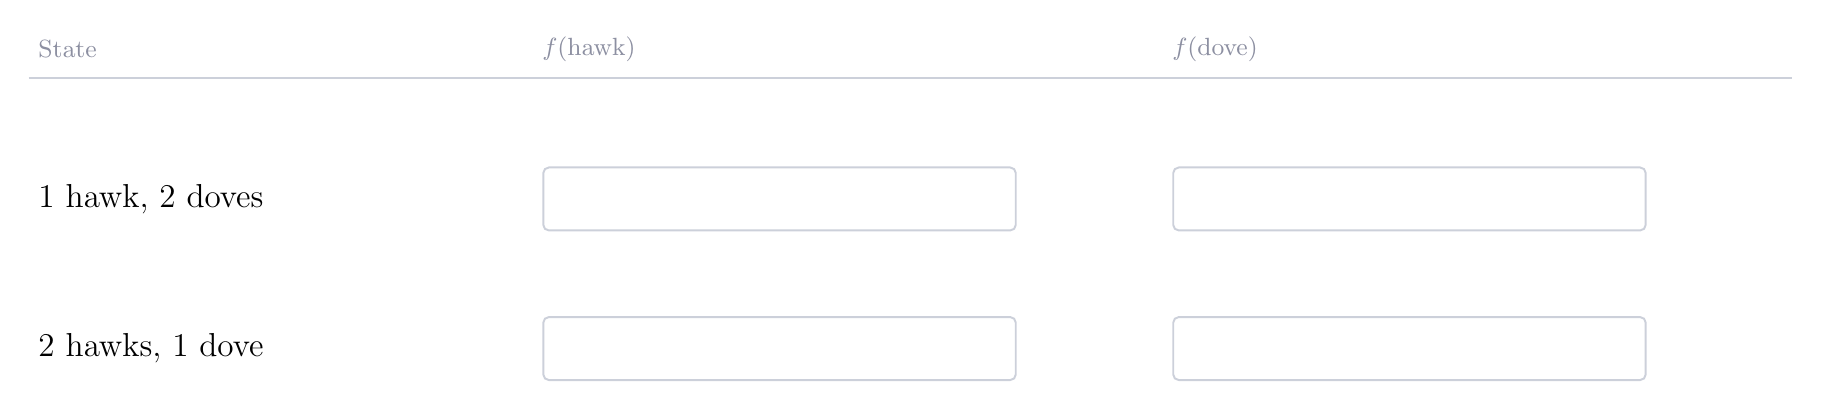
\begin{tikzpicture}[font=\small]
  \foreach \lab/\col in {State/0, {$f(\text{hawk})$}/6.4,
                         {$f(\text{dove})$}/14.4}{%
    \node[anchor=west, text=inkgrey] at (\col,0) {\lab};}
  \draw[inkfaint, line width=0.7pt] (0,-0.36) -- (22.4,-0.36);
  \foreach \state [count=\row from 1] in
    {{1 hawk, 2 doves}, {2 hawks, 1 dove}}{%
    \node[anchor=west, font=\large] at (0,-1.9*\row) {\state};
    \node[anchor=west] at (6.4,-1.9*\row) {\blank[6]};
    \node[anchor=west] at (14.4,-1.9*\row) {\blank[6]};}
\end{tikzpicture}

\vspace{1cm}

{\large Which type is fitter when hawks are rare? \blank[2.6]
\hspace{1.6cm} And when they are common? \blank[2.6]}

\newpage
\slidehead{Who gets born, who dies}

\vspace{0.4cm}

{\large Birth is proportional to fitness. Death is uniform, so it is
proportional to \underline{\hspace{4.5cm}}.}

\vspace{0.7cm}

\hspace{0.3cm}
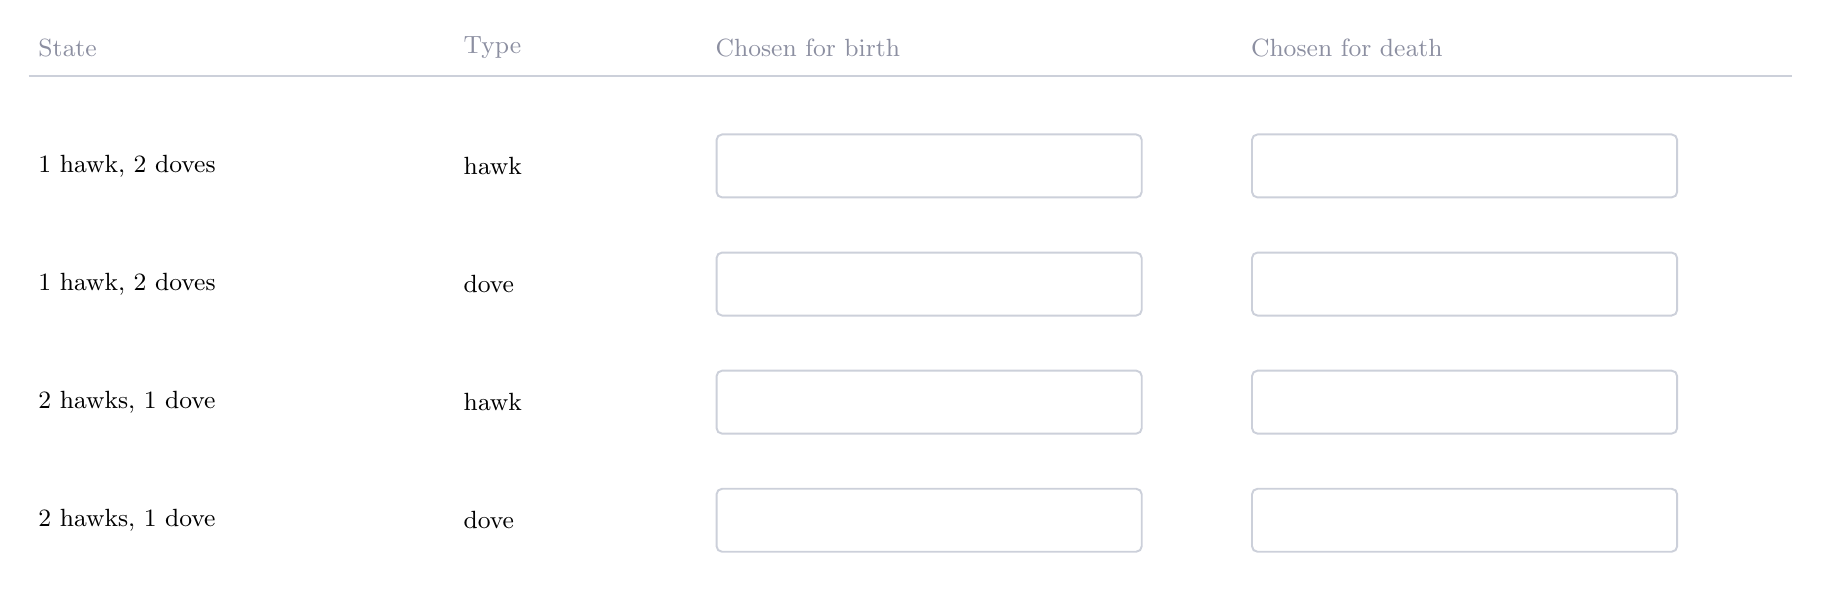
\begin{tikzpicture}[font=\small]
  \foreach \lab/\col in {State/0, Type/5.4, {Chosen for birth}/8.6,
                         {Chosen for death}/15.4}{%
    \node[anchor=west, text=inkgrey] at (\col,0) {\lab};}
  \draw[inkfaint, line width=0.7pt] (0,-0.36) -- (22.4,-0.36);
  \foreach \state/\type [count=\row from 1] in
    {{1 hawk, 2 doves}/hawk, {1 hawk, 2 doves}/dove,
     {2 hawks, 1 dove}/hawk, {2 hawks, 1 dove}/dove}{%
    \node[anchor=west] at (0,-1.5*\row) {\state};
    \node[anchor=west] at (5.4,-1.5*\row) {\type};
    \node[anchor=west] at (8.6,-1.5*\row) {\blank[5.4]};
    \node[anchor=west] at (15.4,-1.5*\row) {\blank[5.4]};}
\end{tikzpicture}

\vspace{0.5cm}

{\small\color{inkgrey} These are the numbers the dice have to reproduce, which
is why we need a four and a six.}

\newpage
\slidehead{Moving between states}

\vspace{0.9cm}

{\large The number of hawks changes only when the type born differs from the
type that dies.}

\vspace{1.1cm}

\begin{center}
{\Large \(p_{10} =\) \blank[2.6] \hspace{1.4cm} \(p_{12} =\) \blank[2.6]
 \hspace{1.4cm} \(p_{21} =\) \blank[2.6] \hspace{1.4cm}
 \(p_{23} =\) \blank[2.6]}
\end{center}

\vspace{1.2cm}

{\large Go back and write these on the chain. What happens with the remaining
probability? \blank[4.4]}

\vspace{0.9cm}

\begin{center}
\workspace{22.6}{2.6}
\end{center}

\newpage
\slidehead{What the room found}

\vspace{0.9cm}

{\large Runs that ended with all hawks: \blank[2.2] out of \blank[2.2],
so a fixation probability of about \blank[2.6].}

\vspace{1.3cm}

{\large The theory says \(x_1 = \dfrac{1}{1 + \gamma_1 + \gamma_1 \gamma_2}\)
with \(\gamma_i = \) \blank[3.4], giving \blank[2.6].}

\vspace{1.3cm}

{\large Close enough? \blank[2.2] \hspace{1.6cm} How many runs would we need to
be sure? \blank[3.4]}

\vspace{1cm}

\begin{center}
\workspace{22.6}{2.4}
\end{center}

\newpage
\slidehead{The same thing, as an exam answer}

\vspace{0.5cm}

{\large What we just did in the room is \textbf{Question 1} on the Moran
Process page, with a population of four instead of three.}

\vspace{0.9cm}

\hspace{0.6cm}
\begin{minipage}{0.92\linewidth}
{\large
\begin{tabbing}
\hspace{1.2cm} \= \hspace{17cm} \= \kill
\textbf{(a)} \> The two random choices made at each step. \> [3]\\[0.55em]
\textbf{(b)} \> Fitnesses with two hawks and two doves. \> [6]\\[0.55em]
\textbf{(c)} \> The probability the number of hawks increases by one. \> [7]\\[0.55em]
\textbf{(d)} \> Define fixation, and say why there are exactly two absorbing
  states. \> [5]\\[0.55em]
\textbf{(e)} \> The probability it decreases, the ratio \(\gamma\), and which
  way it drifts. \> [4]
\end{tabbing}}
\end{minipage}

\vspace{1.2cm}

\begin{center}
{\large\color{inkgrey} vknight.org/gt/topics/moran-process.html}
\end{center}

\end{document}
